%%%%%%%%%%%%%%%%%%%%%%%%%%%%%%%%%%%%%%%%%
% Short Sectioned Assignment
% LaTeX Template
% Version 1.0 (5/5/12)
%
% This template has been downloaded from:
% http://www.LaTeXTemplates.com
%
% Original author:
% Frits Wenneker (http://www.howtotex.com)
%
% License:
% CC BY-NC-SA 3.0 (http://creativecommons.org/licenses/by-nc-sa/3.0/)
%
%%%%%%%%%%%%%%%%%%%%%%%%%%%%%%%%%%%%%%%%%

%----------------------------------------------------------------------------------------
%	PACKAGES AND OTHER DOCUMENT CONFIGURATIONS
%----------------------------------------------------------------------------------------

\documentclass[paper=a4, fontsize=11pt]{scrartcl} % A4 paper and 11pt font size 

\usepackage[T1]{fontenc} % Use 8-bit encoding that has 256 glyphs
\usepackage[english]{babel} % English language/hyphenation
\usepackage{amsmath,amsfonts,amsthm} % Math packages

\usepackage{sectsty} % Allows customizing section commands
%\allsectionsfont{\centering \normalfont\scshape} % Make all sections centered, the default font and small caps

\usepackage{fancyhdr} % Custom headers and footers
\pagestyle{fancyplain} % Makes all pages in the document conform to the custom headers and footers
\fancyhead{} % No page header - if you want one, create it in the same way as the footers below
\fancyfoot[L]{} % Empty left footer
\fancyfoot[C]{} % Empty center footer
\fancyfoot[R]{\thepage} % Page numbering for right footer
\renewcommand{\headrulewidth}{0pt} % Remove header underlines
\renewcommand{\footrulewidth}{0pt} % Remove footer underlines
\setlength{\headheight}{13.6pt} % Customize the height of the header

\numberwithin{equation}{section} % Number equations within sections (i.e. 1.1, 1.2, 2.1, 2.2 instead of 1, 2, 3, 4)
\numberwithin{figure}{section} % Number figures within sections (i.e. 1.1, 1.2, 2.1, 2.2 instead of 1, 2, 3, 4)
\numberwithin{table}{section} % Number tables within sections (i.e. 1.1, 1.2, 2.1, 2.2 instead of 1, 2, 3, 4)

\setlength\parindent{0pt} % Removes all indentation from paragraphs - comment this line for an assignment with lots of text

\usepackage{bbm}
\usepackage{graphicx}
\usepackage{xcolor} % For color
\usepackage{subcaption}
\usepackage{booktabs}

\usepackage{tikz} % For graphs
\usetikzlibrary{positioning}
\usetikzlibrary{calc}

\usepackage{enumerate} % For lettered enumeration
%----------------------------------------------------------------------------------------
%	TITLE SECTION
%----------------------------------------------------------------------------------------

\newcommand{\horrule}[1]{\rule{\linewidth}{#1}} % Create horizontal rule command with 1 argument of height

\title{	
\normalfont \normalsize 
\horrule{0.5pt} \\[0.4cm] % Thin top horizontal rule
\huge Assignment Three \\ % The assignment title
\horrule{2pt} \\[0.5cm] % Thick bottom horizontal rule
}

\author{
	Matthew C.~Scicluna\\
	D\'epartement d'Informatique et de Recherche Op\'erationnelle\\
	Universit\'e de Montr\'eal\\
	Montr\'eal, QC H3T 1J4 \\
	\texttt{matthew.scicluna@umontreal.ca}
}


\date{\normalsize\today} % Today's date or a custom date

\begin{document}

\maketitle % Print the title

%----------------------------------------------------------------------------------------
%	PROBLEM 1
%----------------------------------------------------------------------------------------

\section{DGM}
\begin{minipage}{0.6\textwidth}
	\begin{flushleft}
		Given the following DGM \(G\) the implied factorization for any joint \(p\in\mathcal{L}(G)\) is 
		$$p(X,Y,Z,T)= f_{X}(X)f_{Y}(Y)f_{Z}(Z;X,Y)f_{T}(T;Z)$$ 
		
		It is not true that for any \(p\in\mathcal{L}(G)\) \(X \perp Y \mid T\). For a counterexample, take \(X,Y \sim Bern\left(\frac{1}{2}\right)\), with \(T = Z = X + Y\). Then, $$P(X=1, Y=0 \mid Z=1)=\frac{1}{2}$$ but $$ P(X=1 \mid Z=1)= P(Y=0 \mid Z=1) = \frac{1}{2}$$
		Hence \(X \not\perp Y \mid T\), for this \(p\in\mathcal{L}(G)\), as needed.
	\end{flushleft}
\end{minipage} \hfill
\begin{minipage}{0.35\textwidth}
\begin{flushright}
	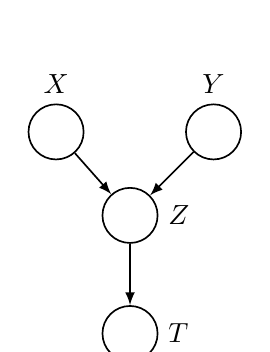
\begin{tikzpicture}[-latex, auto, node distance = 1.5cm and 2cm, on grid, semithick, state/.style ={circle, top color = white, draw, text = black, minimum width=0.7cm}, sh/.style={shade, shading = axis, left color = gray, shading angle = 45}]
	\node[state, label = above:{$X$}] (A) {};
	\node[state, label = above:{$Y$}] (B) [right = of A] {};
	\node[state, label = right:{$Z$}] (C) [below left of = B] {};
	\node[state, label = right:{$T$}] (D) [below = of C] {};
	\path (A) edge node {} (C)
	(B) edge node {} (C)
	(C) edge node {} (D);          
	\end{tikzpicture}
\end{flushright}
\end{minipage}

\section{d-Separation in DGM}
\begin{minipage}{0.6\textwidth}
	\begin{flushleft}
\begin{enumerate}[(a)]
	\item FALSE, consider the path $(C,A), (A,B)$
	\item TRUE
	\item FALSE, consider the path $(C,D), (D,G), (G,B)$
	\item TRUE
	\item FALSE, consider the path $(C,A),(A,B), (B,G)$
	\item FALSE, consider the path $(C,D),(D,G)$
	\item TRUE
	\item FALSE, consider the path $(C,E), (E,H), (H,F), (F,G)$
	\item TRUE
	\item FALSE, consider the path $(B,A), (A,C), (C,D), (D,F), (F,I)$
\end{enumerate}
	\end{flushleft}
\end{minipage} \hfill
\begin{minipage}{0.35\textwidth}
	\begin{flushright}
		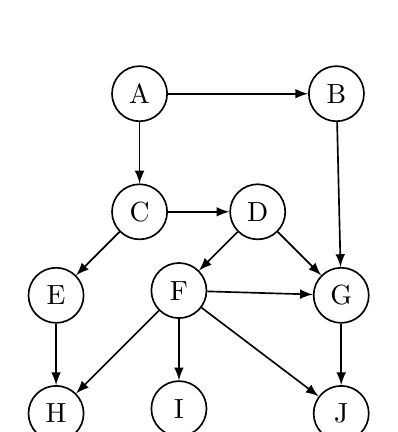
\begin{tikzpicture}[-latex, auto, node distance = 1.5cm and 2cm, on grid, semithick, state/.style ={circle, top color = white, draw, text = black, minimum width=0.7cm}, sh/.style={shade, shading = axis, left color = gray, shading angle = 45}]
		\node[state] (A) {A};
		\node[state] (B) [right = 2.5cm of A] {B};
		\node[state] (C) [below = of A] {C};
		\node[state] (E) [below left = 1.5cm of C] {E};
		\node[state] (D) [right = 1.5cm of C] {D};
		\node[state] (F) [below left = 1cm and 1cm of D] {F};
		\node[state] (G) [below right = 1.5cm of D] {G};
		\node[state] (H) [below = of E] {H};
		\node[state] (I) [below = of F] {I};
		\node[state] (J) [below = of G] {J};
		\path (A) edge node {} (C)
		(A) edge node {} (B)
		(B) edge node {} (G)
		(C) edge node {} (E)
		(C) edge node {} (D)
		(D) edge node {} (F)
		(D) edge node {} (G)
		(E) edge node {} (H)
		(F) edge node {} (G)
		(F) edge node {} (H)
		(F) edge node {} (I)
		(F) edge node {} (J)
		(G) edge node {} (J);          
		\end{tikzpicture}
	\end{flushright}
\end{minipage}

\section{Positive interactions in-V-structure}
Given \(X,Y,Z\) binary RV's with a joint distribution parameterized by $X \rightarrow Z \leftarrow Y$, with $a=P(X=1), b=P(X=1|Z=1), c=P(X=1|Z=1,Y=1)$.
We notice that if we set $X \sim Bern\left(\frac{1}{2}\right)$, $Y \sim Bern\left(\frac{1}{2}\right)$ and if we denote $\alpha=P(Z=1\mid X=1,Y=1), \beta=P(Z=1\mid X=1,Y=0), \gamma=P(Z=1\mid X=0,Y=1)$ and $\delta = P(Z=1\mid X=0,Y=0)$ that we have, by cancellation of marginal probabilities of $X$ and $Y$, that $c-b = \frac{\alpha}{\alpha + \gamma} - \frac{\alpha + \beta}{\alpha + \beta + \gamma + \delta}$. We then set $\alpha, \beta, \gamma, \delta$ accordingly to satisfy the inequality relations between $a$, $b$ and $c$ with fixed $a=\frac{1}{2}$.
\begin{enumerate}[(a)]
	\item \begin{enumerate}[(i)]
			\item $X \sim Bern\left(\frac{1}{2}\right)$, $Y \sim Bern\left(\frac{1}{2}\right)$ and $Z = 1 - X \oplus Y$. Then $a=\frac{1}{2}$ but $c=0$
			
				
			\item Again, we fix $X \sim Bern\left(\frac{1}{2}\right)$, $Y \sim Bern\left(\frac{1}{2}\right)$ and $Z$ has the following probability table:
			\begin{center}
				\begin{tabular}{*3l}  
					\toprule
					X & Y & P(Z=1) \\ \midrule
					0 & 0 & 0.1\\
					0 & 1 & 0.8\\
					1 & 0 & 1\\
					1 & 1 & 1	
					\\\bottomrule
					\end{tabular}
			\end{center}
				Then $a=\frac{1}{2}$, $c=\frac{\frac{1}{2}}{0.8 + 0.2\frac{1}{2}}=\frac{5}{9}$ and $b=\frac{\frac{1}{2}}{0.83 + 0.17\frac{1}{2}}\approx0.855$, and $a<c<b$.
			\item  Again, we fix $X \sim Bern\left(\frac{1}{2}\right)$, $Y \sim Bern\left(\frac{1}{2}\right)$ and $Z$ has the following probability table:
			\begin{center}
				\begin{tabular}{*3l}  
					\toprule
					X & Y & P(Z=1) \\ \midrule
					0 & 0 & 1\\
					0 & 1 & 0.8\\
					1 & 0 & 0\\
					1 & 1 & 1	
					\\\bottomrule
				\end{tabular}
			\end{center}
			Then $a=\frac{1}{2}$, $c=\frac{1}{1.8}$ and $b=\frac{1}{2.8}$, and $b<a<c$.
			
			\end{enumerate}
			
	\item \begin{enumerate}[(i)]
		\item The semantic here is that $Z$ is a negated XOR gate for $X$ and $Y$.
		Hence, knowing that both $Y$ and $Z$ are ``on'' means that $X$ must not be.
		\item Semantically, $Z$ will certainly be ``on'' if $X$ is, and probably will be ``on'' if $Y$ is. So $Z$ being ``on'' gives evidence for $X$, but having $Y$ ``on'' as well can explain away $Z$ (i.e. it is more likely that $Z$ was caused by only $Y$).
		\item Semantically, $Z$ is likely to be ``on'' unless $X$ is ``on'' and $Y$ isn't. So if $Z$ is ``on'', $X$ is less likely to be, since $Y$ would have to be ``on'' too.
		  \end{enumerate}	
\end{enumerate}

\section{Flipping a covered edge in a DGM}
Let $G = (V, E)$ be a DAG. We say that a directed edge $(i, j) \in E$ is a covered edge if and only
if $\pi_j = \pi_i \cup \{i\}$. Let $G' = (V, E')$, with $E' = (E-\{(i, j)\}) \cup \{(j, i)\}$. Prove that $\mathcal{L}(G) = \mathcal{L}(G')$.
\\

PROOF: Fix $i,j, G$ and $E$. Denote \(\pi'_k\) as the set of parents for a node $k$ under $E'$. We note that \(\pi'_k = \pi_k\) for \(k\ne i,j\) and \(\pi'_i = \pi_i \cup \{j\}\) and \(\pi'_j = \pi_i\).

For the forward direction we let $p \in \mathcal{L}(G)$. 
We want to show that \(p(x_v)=\prod_{k=1}^{n}p(x_k|x_{\pi'_k})\)

Notice that: 
\begin{align}
p(x_v)&=\prod_{k\ne i,j}p(x_k|x_{\pi_k})P(x_i|x_{\pi_i})P(x_j|x_{\pi_i}, x_i) \\
&= \prod_{k\ne i,j}p(x_k|x_{\pi_k})P(x_i, x_j|x_{\pi_i}) \\
&= \prod_{k\ne i,j}p(x_k|x_{\pi_k})P(x_j|x_{\pi_i})P(x_i|x_{\pi_i}, x_j) \\
&= \prod_{k\ne i,j}p(x_k|x_{\pi'_k})P(x_j|x_{\pi'_j})P(x_i|x_{\pi'_i})\\
&=\prod_{k=1}^{n}p(x_k|x_{\pi'_k})
\end{align}

As needed. For the reverse direction, let $p \in \mathcal{L}(G')$
\begin{align}
p(x_v)&=\prod_{k\ne i,j}p(x_k|x_{\pi'_k})P(x_i|x_{\pi'_j}, x_j)P(x_j|x_{\pi'_j}, x_i) \\
&= \prod_{k\ne i,j}p(x_k|x_{\pi'_k})P(x_i|x_{\pi_i})P(x_j|x_{\pi_i}, x_i) \\
&= \prod_{k\ne i,j}p(x_k|x_{\pi_k})P(x_i|x_{\pi_i})P(x_j|x_{\pi_j})
\end{align}

And (4.5) and (4.8) complete the proof.

\section{Equivalence of directed tree DGM with undirected tree UGM}

Let \(G\) be a directed tree and \(G'\) be its corresponding undirected tree. Prove that $\mathcal{L}(G) = \mathcal{L}(G')$.
\\

PROOF: For the forward direction we set the edge potentials \(\psi_{(i,j)}(x_i,x_j) = P(x_j|x_i)\). For the node potentials we set \(\psi_r(x_r) = P(x_r)\), where \(x_r\) is the root of the tree, and 1 for the rest. It is clear that 
\begin{align*}
P(x_v)=\prod_{i \in V} P(x_i | x_{\pi_i})=\psi_r(x_r)\prod_{(\pi_i,i)\in E}\psi_{(\pi_i,i)}(x_{\pi_i}, x_i)
\end{align*}
 We note that $Z=1$ since
\begin{align*}
Z&=\sum_{x_v}\psi_r(x_r)\prod_{(\pi_i,i)\in E}\psi_{(\pi_i,i)}(x_{\pi_i}, x_i)\\
&=\sum_{x_r}\psi_r(x_r)\prod_{(\pi_i,i)\in E}\sum_{x_i}\psi_{(\pi_i,i)}(x_{\pi_i}, x_i) \\
&=\sum_{x_r}P(x_r)\prod_{(\pi_i,i)\in E}\sum_{x_i}P(x_i | x_{\pi_i}) = 1
\end{align*}

For the reverse direction, TBD

\newpage

\section{Hammersley-Clifford Counter example}

Given $P(0,0,0,0)=P(1,0,0,0)=P(1,1,0,0)=P(1,1,1,0)=P(0,0,0,1)=P(0,0,1,1)=P(0,1,1,1)=P(1,1,1,1)=\frac{1}{8}$ and the following graph:

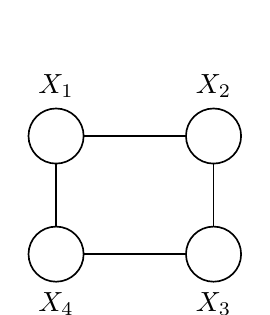
\begin{tikzpicture}[auto, node distance = 1.5cm and 2cm, on grid, semithick, state/.style ={circle, top color = white, draw, text = black, minimum width=0.7cm}, sh/.style={shade, shading = axis, left color = gray, shading angle = 45}]
\node[state, label = above:{$X_1$}] (A) {};
\node[state, label = above:{$X_2$}] (B) [right = of A] {};
\node[state, label = below:{$X_3$}] (C) [below = of B] {};
\node[state, label = below:{$X_4$}] (D) [left = of C] {};
\path (A) edge node {} (B)
(B) edge node {} (C)
(C) edge node {} (D)
(D) edge node {} (A);          
\end{tikzpicture}

We want to show that \(p \notin \mathcal{L}(G)\).
\\

PROOF: Suppose \(p \in \mathcal{L}(G)\), then there are \(\psi\) potentials such that \begin{align*}
P(x_1,x_2,x_3,x_4)=\psi_{x_1,x_2}(x_1,x_2)\psi_{x_2,x_3}(x_2,x_3)\psi_{x_3,x_4}(x_3,x_4)\psi_{x_4,x_1}(x_4,x_1)
\end{align*}

Notice that $P(0,1,0,0)=0$ implies that at least one of the following must be $0$:
$\psi_{x_1,x_2}(0,1)$,
$\psi_{x_2,x_3}(1,0)$,
$\psi_{x_3,x_4}(0,0)$,
$\psi_{x_4,x_1}(0,0)$
\\

We notice that if $\psi_{x_1,x_2}(0,1)=0$ then $P(0,1,1,1)=0$ which contradicts that $P(0,1,1,1)=\frac{1}{8}$. Similarily, if $\psi_{x_2,x_3}(1,0)=0$ then $P(1,1,0,0)=0$, contradicting that it is \(\frac{1}{8}\). The same reasoning shows why $\psi_{x_3,x_4}(0,0) \ne 0$. Finally, if $\psi_{x_4,x_1}(0,0)=0$ then $P(0,0,0,0)=0$, which again is a contradiction.

\label{key}

\end{document}